\documentclass[conference]{IEEEtran}
\IEEEoverridecommandlockouts
% The preceding line is only needed to identify funding in the first footnote. If that is unneeded, please comment it out.
\usepackage{cite}
\usepackage{amsmath,amssymb,amsfonts}
\usepackage{algorithmic}
\usepackage{graphicx}
\usepackage{textcomp}
\usepackage{xcolor}
\def\BibTeX{{\rm B\kern-.05em{\sc i\kern-.025em b}\kern-.08em
    T\kern-.1667em\lower.7ex\hbox{E}\kern-.125emX}}
\begin{document}

\title{Modeling and simulation of Power Consumption on Heterogenous CPU Cores under varying workloads and operating conditions\\

}

\author{\IEEEauthorblockN{Atharv Arun Desai}
\IEEEauthorblockA{\textit{Department of CSA} \\
\textit{Indian Institute of Science (IISc)}\\
Bangalore, India\\
atharvarun@iisc.ac.in}
\and
\IEEEauthorblockN{Boul Chandra Garai}
\IEEEauthorblockA{\textit{Department of CSA} \\
\textit{Indian Institute of Science (IISc)}\\
Bangalore, India \\
chandraboul@iisc.ac.in}
\and
\IEEEauthorblockN{Himanshu Srivastava}
\IEEEauthorblockA{\textit{Department of CSA} \\
\textit{Indian Institute of Science (IISc)}\\
Bangalore, India\\
himanshusriv@iisc.ac.in}
\and
\IEEEauthorblockN{Vaisakh P S}
\IEEEauthorblockA{\textit{Department of CSA} \\
\textit{Indian Institute of Science (IISc)}\\
Bangalore, India\\
vaisakhp@iisc.ac.in}
}

\maketitle

\begin{abstract}
    This document serves as phase-1 report for E0-240 - Modeling and Simulation course project delivery. The main objective of this project is to apply concepts learned in E0-240 course in to Modeling and simulation of a real-world system, which in this case is Multi-core, Heterogenous CPU. This project, will focus on developing a Power Consumption Model for simulated Full-System \cite{8718630} under varying workloads. This model will be developed taking in consideration various operating conditions of the CPU such as Dynamic Frequency Scaling, Heterogenous Cores \cite{arm-big.little-whitepaper}
\end{abstract}

\begin{IEEEkeywords}
    Modeling, simulation, heterogenous CPU cores, power consumption
\end{IEEEkeywords}

%% ---------------------------------------------------------------------------------------------------------
%% Background 
%%    - Motivation behind the work
%%    -  any technical background (any special definition/technology which is a required knowledge to 
%%       understand the rest of the document)
%%    - existing work in the domain etc. 
\section{Background}
%% ---------------------------------------------------------------------------------------------------------


%% ---------------------------------------------------------------------------------------------------------
\section{Methodology}
%% ---------------------------------------------------------------------------------------------------------
    \par As mentioned in previous work \cite{Reddy2017EmpiricalCP}, a similar method is followed, wherein a ODROID-XU4\cite{odroid-xu4} Big-Little development board is chosen as first target for experimentation, data gathering and validation efforts. An overview of this hardware is show in Figure. \ref{fig-odroid-hwoverview}. 

    \begin{figure}[b]
        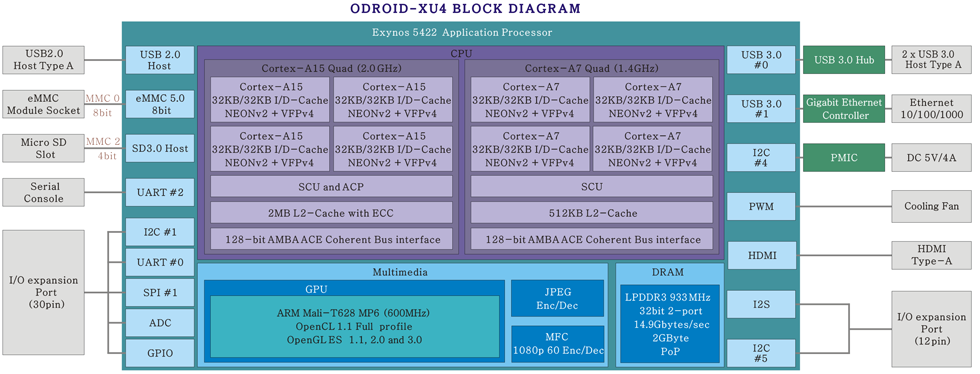
\includegraphics{rsrc/201506191222574523.png}
        \caption{ODroid XU4 board overview}
        \label{fig-odroid-hwoverview}
    \end{figure}
    
    \subsection{Data Gathering}
        \par test


        \begin{figure}[t]
            \centering
            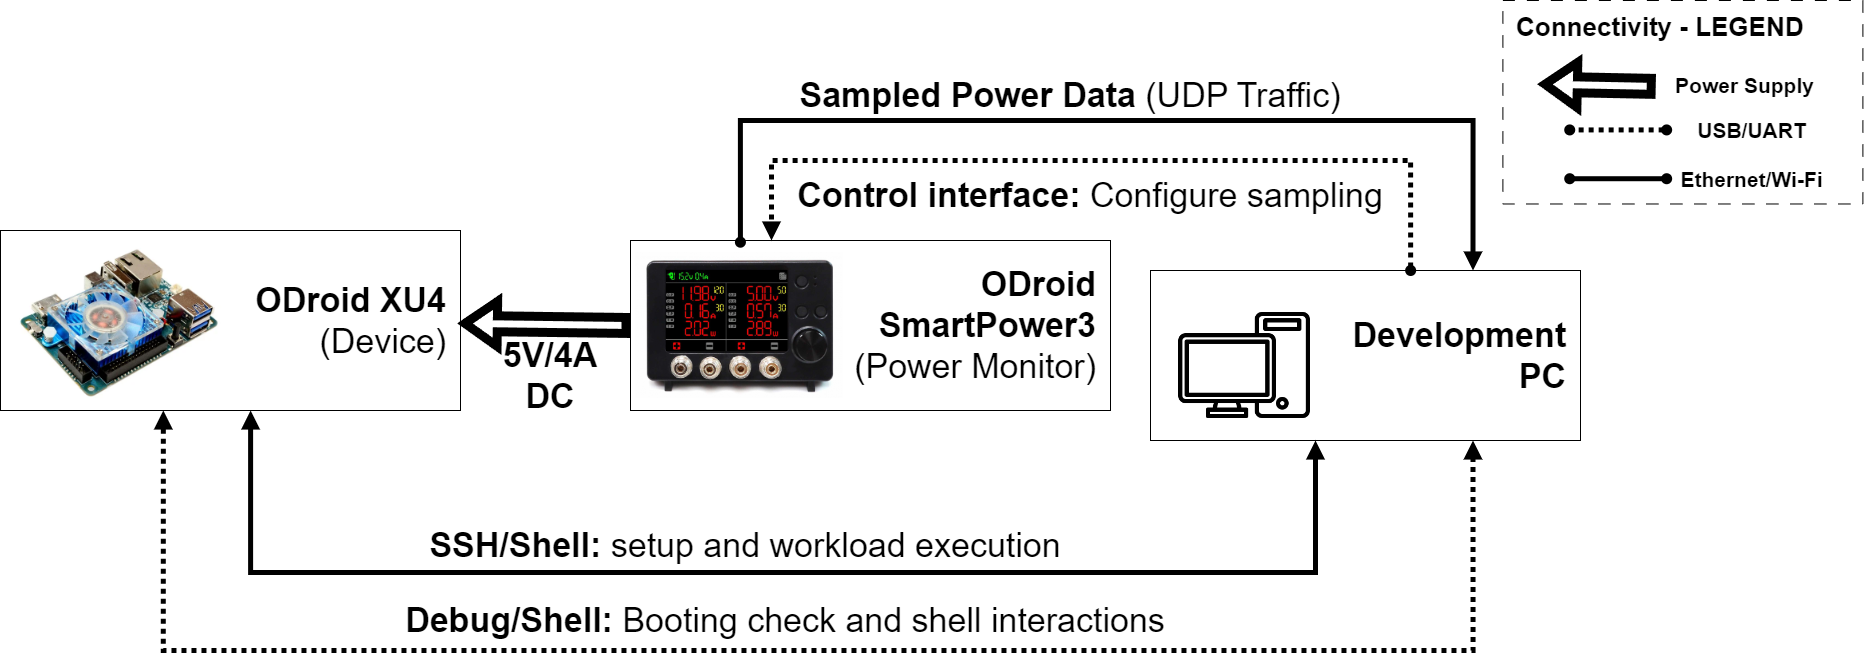
\includegraphics[width=0.48\textwidth]{rsrc/Experiment-setup.drawio.png}
            \caption{Experiment setup for power data gathering from ODROID-XU4\cite{odroid-xu4} hardware}
            \label{fig-Experiment-setup}
        \end{figure}


        \begin{table}[htbp]
            \caption{Power and Performance Feature gathered from mentioned experiment setup}
            \begin{center}
                \begin{tabular}{|c|p{1.8cm}|p{3.9cm}|}
                    \hline
                    \textbf{Feature/Statistics}&\multicolumn{2}{|c|}{\textbf{Feature details }} \\
                    \cline{2-3} 
                    \textbf{Type} & \multicolumn{1}{|c|}{\textbf{\textit Source}} & \multicolumn{1}{|c|}{\textbf{\textit Details}} \\
                    \hline
                    CPU Clock Cycles  & perf[x]  & CPU cycles, us cycles, instructions, CPU frequency, CPU idle state statistics \\
                    \hline
                    Instruction Branches  & perf[x]  & Branch instruction and speculative operation statistics \\
                    \hline
                    Caches   & perf[x]  & Data/Instruction cache references, misses at L1, Last-Level-Cache levels  \\
                    \hline
                    Board Level Power & SmartPower3\cite{odroid-smartpower3} & Current, Power drawn from power supply. \\
                    \hline
                    Misc. Performance  & perf[x]  & CPU Migrations, Context switches, Virtual memory \\
                    \hline
                \end{tabular}
                \label{Power-Perf-data-gathered}
            \end{center}
        \end{table}

        \begin{table}[htbp]
            \caption{List of workloads being used for data gathering and validation}
            \begin{center}
                \begin{tabular}{|c|p{4cm}|c|}
                    \hline
                    \textbf{Workload}&\multicolumn{2}{|c|}{\textbf{Workload details and status  of integration}} \\
                    \cline{2-3} 
                    \textbf{Type} & \multicolumn{1}{|c|}{\textbf{\textit Workloads}} & \textbf{\textit{Status}} \\
                    \hline
                    Stress Test & stress command \cite{linux-stress-testing} & $\checkmark$ \\
                    \hline
                    Video Encoding & ffmpeg encode \cite{linux-stress-testing} & $\checkmark$ \\
                    \hline
                    File Compression & gzip, bzip2, xz on complex datasets \cite{compression-benchmarking} & $\checkmark$ \\
                    \hline
                    Benchmark Suite & SPEC2017 CPU Benchmarks \cite{10.1145/3185768.3185771} & Planned \\
                    \hline
                \end{tabular}
                \label{Workload-listing}
            \end{center}
        \end{table}

%% ---------------------------------------------------------------------------------------------------------
\section{Phase-2 Progress}
%% ---------------------------------------------------------------------------------------------------------
    \par test

%% ---------------------------------------------------------------------------------------------------------
\section{Phase-2 Observations and Results}
%% ---------------------------------------------------------------------------------------------------------
    \par test

%% ---------------------------------------------------------------------------------------------------------
\section{Discussion on Phase-2 outcomes}
%% ---------------------------------------------------------------------------------------------------------

%% ---------------------------------------------------------------------------------------------------------
\section{Next Step}
%% ---------------------------------------------------------------------------------------------------------

    \subsection{Modeling and Empirical Model generation}

    \subsection{Power Model Integration to Gem5}





% ------------------------------------------------------------------------------
% Reference and Cited Works
% ------------------------------------------------------------------------------
\bibliographystyle{IEEEtran}
\bibliography{references.bib}

% ------------------------------------------------------------------------------

\end{document}
